\documentclass[journal]{IEEEtran}
\IEEEoverridecommandlockouts

\renewcommand\IEEEkeywordsname{Palabras Clave}

\usepackage[spanish]{babel}
\usepackage[utf8x]{inputenc}
\usepackage{cite}
\usepackage{amsmath,amssymb,amsfonts}
\usepackage{algorithmic}
\usepackage{graphicx}
\usepackage{textcomp}
\usepackage{xcolor}
\usepackage{fancyhdr}
\usepackage{listings}
\usepackage{float}
\usepackage{blindtext}
\usepackage{newtxmath}
\usepackage{wrapfig}
\usepackage{mathtools}
\usepackage{breqn}

\lstdefinestyle{code}{%
backgroundcolor=\color{gray!5},
basicstyle=\ttfamily\small,
commentstyle=\color{green!60!black},
keywordstyle=\color{magenta},
stringstyle=\color{blue!50!red},
showstringspaces=false,
%captionpos=b,
numbers=left,
numberstyle=\footnotesize\color{gray},
numbersep=8pt,
%stepnumber=2,
tabsize=2,
%frame=L,
%framerule=1pt,
%rulecolor=\color{red},
breaklines=true,
}

\def\BibTeX{{\rm B\kern-.05em{\sc i\kern-.025em b}\kern-.08em
    T\kern-.1667em\lower.7ex\hbox{E}\kern-.125emX}}


\graphicspath{ {../Imagenes/} }

\begin{document}
    \title{Simulador Dinámico de un Exoesqueleto de 6GdL\\
    \small{Reporte de Medio Término}}

    \author{\IEEEauthorblockN{García-Álvarez Gregorio E. , Luna-Macías Antonio J. , Tevera-Ruiz Alejandro\\}
    \IEEEauthorblockA{\textit{Departamento: Roobótica y Manufactura Avanzada} \\
    \textit{Centro de Investigación y de Estudios Avanzados (CINVESTAV)}}
    }

    \maketitle

    \begin{abstract}
        El presente documento describe el desarrollo cinemático y dinámico que simula un exoesqueleto
        con 6 grados de libertad (GDL).
        \noindent El diseño está enfocado para utilizarse en el dedo índice, sin embargo debido a que
        este trabajo aún no incorpora otras cadenas cinemáticas, como el diseño original presentado en
        el trabajo: "HEXOTRAC"[1], esto implica que el propio, se pueda utilizar adecuadamente en
        cualquier dedo a excepción del pulgar. 
        \noindent Una de las características que tendrá el exoesqueleto presentado, será que el dedal
        distal, tendrá capacidades hápticas y estará actuado en todos sus grados de libertad,
        sin embargo por el momento, no es el alcance concerniente a este documento.         
    \end{abstract}

    \begin{IEEEkeywords}
    Simulador, Exoesqueleto, GRyMA
    \end{IEEEkeywords}

    \section{Introducción}

    \blindtext[0]

    \section{Descripción Metodológica}

    El diseño del dedo exoesqueleto con 6 GDL se muestra en la Figura \ref{fig:Diseno3D} en su 
posición inicial de "CASA" y está constituido por una cadena cinemática de 7 eslabones, que 
están todos conectados entre sí por articulaciones revolutas. El software que se utilizó para 
generar el diseño en 3D, fue solidworks porque tiene varias herramientas que ayudaron en el 
desarrollo matemático, así como su versatilidad para enlazarse con matlab, software con el que 
se programaron los cálculos.  

\begin{figure}[H]
    \centering
    \includegraphics[scale=0.2]{Dedo Vist Isometrica.png} 
    \caption{Diseño 3D}
    \label{fig:Diseno3D}
\end{figure}

La disposición de las articulaciones que se muestran en la Figura \ref{fig:EsqArtOri}, fueron las 
planteadas en el trabajo HEXOTRAC: A highly Under-Actuated Hand Exoskeleton for Finger Tracking 
and Force Feedback (REFERENCIA).

\begin{figure} [H]
    \centering
    \includegraphics[scale=0.4]{EsquemaArticulaciones.png} 
    \caption{Esquema de las Articulaciones Original}
    \label{fig:EsqArtOri}
\end{figure}

Sin embargo por el equipo propuso una modificación y se agregó un eslabón más, de esta manera 
se evita que la articulación revoluta  $q_{14}$ y  $q_{15}$ estuvieran fusionadas, como se 
visualiza en la Figura \ref{fig:EsqArtOri}. El dibujo posicionado con una perspectiva lateral 
derecha, que se visualiza en la Figura \ref{fig:ExoPara} proporciona una imagen con dimensiones 
parametrizadas, mismas que se plasman en la siguiente tabla: 

\begin{table}[!ht] %[H]
    \centering
    \begin{center}
        \begin{tabular}{ccc}
        Parámetros & [m] \\
        \hline \hline 
        L1 & 0.03235525  \\ 
        L2 & 0.10513390  \\
        L3 & 0.02462267  \\
        L4 & 0.02228474  \\
        L5 & 0.04334075  \\
        L6 & 0.00600000  \\
        L7 & 0.01999013  \\
        L8 & 0.02565247  \\
        L9 & 0.01273194  \\
        L10 & 0.03641522 \\
        \end{tabular}
    \end{center}
\end{table}

Cabe destacar que el ángulo $\alpha$ que aparece en la imagen \ref{fig:ExoPara} es 
$\alpha$ = 59.26721315 [rad]. En la misma figura \ref{fig:ExoPara} se aprecia la asignación 
de referenciales $\Sigma_0$, $\Sigma_1$, $\Sigma_2$, $\Sigma_3$, $\Sigma_4$, $\Sigma_5$,  
$\Sigma_6$ y $\Sigma_7$. Los marcos inerciales propuestos a cada GdL se colocaron utilizando 
la convención GRyMA, manteniendo la dirección positiva de la mano derecha.

También se asignaron materiales, proponiendo para los eslabones un polímero termoplástico de 
nombre "acrilonitrilo butadieno estreno" también conocido como filamento ABS, utilizado por 
impresoras 3D, pensando que en un futuro próximo podamos imprimir el modelo y así experimentar 
con el en un entorno real. En el caso del dedal, se seleccionó un polímero artificial que 
pertenece al grupo de las poliamidas, llamado comunmente "Nylon", pues creemos que para cuidar 
la comodidad del usuario, al ingresar su dedo, el material no debe ser tan rígido y el nylon 
permite un equilibrio entre la suavidad y al mismo tiempo que no sea deformable.

Finalmente los motores propuestos son de micro Metal LP con reductora de 50:1, de corriente 
continua, con dimensiones de 24 x 10 x 12 mm y 10 gramos de peso. 

Al proponer materiales específicos, conocer sus dimensiones e incorporar las masas del motor 
pololu, se puede conocer el peso total del exoesqueleto, así como sus centros de masa 
(REFERENCIA TABLA 1 ANEXOS ) y los tensores de inercia de cada eslabón 
(REFERENCIA MATRICES EN ANEXOS), esta información se encuentra descrita en la sección de ANEXO  

\begin{figure}[H]
    \centering
    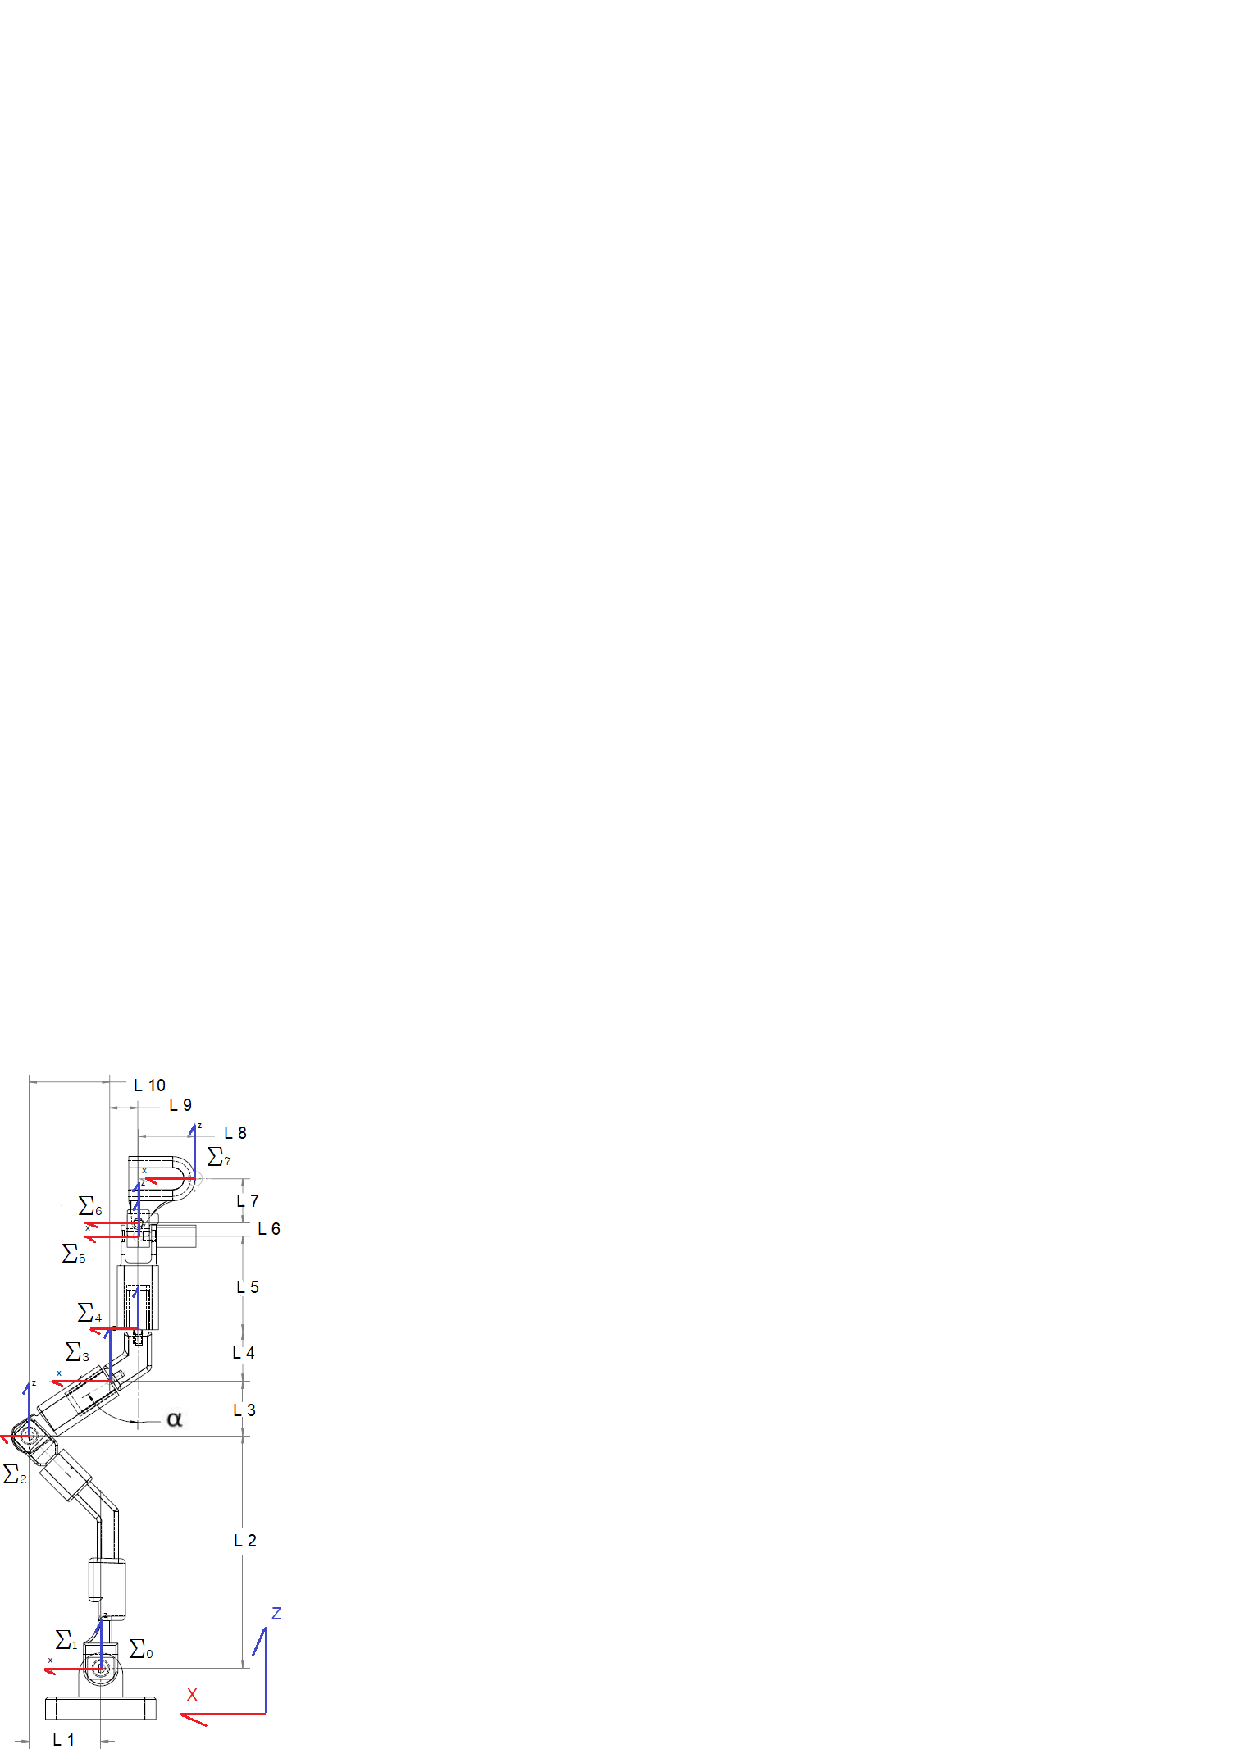
\includegraphics[scale=0.7]{ExoParametrizado.png}
    \caption{Esquema de las Articulaciones Utilizado}
    \label{fig:ExoPara}
\end{figure}

Conocer la cantidad de grados de libertar que tiene el exoesqueleto, nos servirá para identificar 
la versatilidad del movimiento que se podrá ejercer. Existen 3 clasificaciones [2]:

\begin{itemize}
    \item Menos de 6 GDL.  si el robot está diseñado para moverse en un espacio tridimensional, presentará  limitaciones su movimiento. 
    \item Exactamente 6 GDL. Se podrá mover de manera independiente en cada uno de los seis parámetros que conforman el espacio de trabajo tridimensional.
    \item Más de 6 GDL. Si un robot tiene más actuadores que los parámetros del espacio, implica que está sobre actuado.
\end{itemize}


    \subsection{Cinemática directa}

    \noindent La cinemática directa consiste en definir la posición y orientación del efector final, en función de las
    coordenadas generalizadas de cada articulación, con respescto a un marco de referencia [3], en este caso particular,
    es un marco de referencia no inercial.

    Para lograrlo, se requieren cadenas cinemáticas desde el referencial base hasta el referencial local; para cada uno de
    estos ejes coordenados, se requiere el cálculo de matrices de transformación homogéneas mismas que definen el movimiento
    de rotación y traslación en función de donde se ubique el marco referencial de cada articulación. 

    Debido a que cada eslabón tiene asignada una coordenada generalizada y por lo tanto, tiene su propia matriz que describe
    su movimiento, se necesita multiplicar cada una de las matrices de transformación homogéneas.
    \\
    La matriz de transformación homogenea tiene la siguiente forma:
    \begin{equation*} A_i = 
        \begin{bmatrix}
        R^i_{i-1} & d^i_{i-1}\\
        0 & 1
        \end{bmatrix}
    \end{equation*}
    \noindent Cabe destacar que la matriz $R^j_i \in \mathbb{R}^{3\times 3}$ representa la orientación del referencial $j$
    respecto al referencial $i$, y el vector $d^j_{i}$ expresa la traslación del referencial $j$ respecto al referencial $i$.\\

    \noindent Existen diferentes métodos para asignar los referenciales de coordenadas generalizadas, y así obtener la matriz
    de transformación homogenea; uno de los más utilizados en robótica industrial es el denominado: "Denavit Hartenberg",
    pero no es el único. En el curso se presentan 2 más (Denavit Hartenberg modificado "mDH" y GRyMA), lo cierto es que los
    3 buscan reducir la cantidad de parámetros que se requieren para definir las transformaciones homogéneas entre marcos
    referenciales. 

    \noindent Los movimientos rígidos generales se definen mediante una traslación $d \in \mathbb{R}^3$ y una rotación
    $R \in SO(3)$. Por tanto, se componen de 6 GDL para cada par de marcos referenciales consecutivos. La asignación del marco
    para cada elemento rígido da como resultado todos los $A_i (q_i) \in SE(3)$ en el sistema.

    \noindent Dos de los ejemplos más comunes son las convenciones clásicas de Denavit-Hartenberg (DH) y las modificadas de
    Denavit-Hartenberg (mDH). Ambos reducen los parámetros requeridos de 6 a 4, lo que da como resultado la torsión del enlace
    ($\alpha$), la longitud del enlace ($a$), el ángulo de unión ($\theta$) y el desplazamiento del enlace ($d$).
    \noindent A continuación se presentarán las reglas que se deben llevar a cabo para la asignación de referenciales,
    correspondiente.

    \subsubsection{Denavit Hartenberg}
    \noindent Existen dos restricciones al momento de definir del marco de referencia: 
    \begin{enumerate}
        \item El eje $x$ de un referencial dado debe ser perpendicular al eje $z$ de los referenciales vecinos consecutivas. 
        \item El eje $x$ de un referencial dado y el eje $z$ del referencial vecino consecutivo deben intersectar. 
    \end{enumerate}

    \noindent Debido a que la convención DH define una secuencia intrínseca explícita:
    $\theta_i \rightarrow d_i \rightarrow a_i \rightarrow \alpha_i$, las transformaciones homogéneas $A_i (q_i)$,
    que representan el movimiento rígido correspondiente, se obtiene la siguiente forma particular:
    \begin{align*}
        A_i (q_i) & \triangleq A_R (R_{z,\theta}) A_T (d_i k) A_T (a_i i) A_R (R_{x,\alpha_i}) \\
        & = \left[  \begin{array}{cc}
            R_{i-1}^i (\cdot)  & d_{i/i-1}^{(i-1)} (\cdot) \\
            0 & 1  
    \end{array} \right]
    \end{align*}
    donde
    \begin{align*}
        R_{i-1}^i (\cdot) & = R_{z,\theta_i}  R_{x,\alpha_i} \\ 
        & = \left[  \begin{array}{ccc}
            \cos{\theta_i}  & -\sin{\theta_i}\cos{\alpha_i} & \sin{\theta_i} \sin{\alpha_i} \\
            \sin{\theta_i} &  \cos{\theta_i}\cos{\alpha_i} &
            -\cos{\theta_i}\sin{\alpha_i} \\
            0 & \sin{\alpha_i} & \cos{\alpha_i}
        \end{array} \right]
    \end{align*}

    \vspace{2mm}
    \begin{equation*}
    \begin{array}{ccc}
        d_{i/i-1}^{(i-1)} (\cdot) & = d_i k + a_i R_{z,\theta_i} R_{x,\alpha_i}  i 
        & = \left[  \begin{array}{c}
            a_i \cos{\theta_i} \\
            a_i \sin{\theta_i} \\
            d_i 
        \end{array} \right]
    \end{array}
    \end{equation*}

    \vspace{5mm}
    \noindent Además se sabe que solo uno de los parámetros DH es variable en el tiempo, por lo tanto existen
    variaciones en el ángulo de articulación o en el desplazamiento del enlace\\
    \vspace{-2mm}
    \begin{equation*}
        \begin{array}{cc}
            \theta_i (t) = \theta_{i_0} + q_i (t) & \text{Articulación Revoluta} (R) \\
            d_i (t) = d_{i_0} + q_i (t) & \text{Articulación presmática} (P)
        \end{array}
    \end{equation*}
    \vspace{1mm}
    \noindent La cinemática directa de un robot manipulador puede ser determinada por la multiplicación de todas
    las matrices $A_i (q_i)$ obtenidas por la tabla de los parámetros de DH. 

    \noindent Sabiendo que el exoesqueleto tiene asignados 6 coordenadas generalizadas $q_i$ se tendría que
    aplicar la multiplicación de la siguiente manera:
    \begin{equation*}
        % Revisar porque le moví a los subíndices jeje Atte. Alejandro :)
    A = A_1(q_1) \hspace{1mm} A_2(q_2) \hspace{1mm} A_3(q_3) \hspace{1mm} A_4(q_4) \hspace{1mm} A_5(q_5)
        \hspace{1mm} A_6(q_6) \hspace{1mm} A_7(q_7)
    \end{equation*}
    \noindent Sin embargo, esto no es del todo cierto, debido a que para lograr cumplir con las 2 condiciones que
    estipula la metodología, aunado a la forma que tiene el diseño de los eslabones 1 y 3, implica que se generen
    referenciales virtuales.     \\ 
    \noindent Después de comparar los resultados de la matriz homogenea obtenida por las 3 metodologías y comparando
    los resultados de las mismas, se optó por no utilizar la metodología tradicional y llevar acabo los cálculos con
    el siguiente método: \\ 
    \subsubsection{GRyMA}
    \noindent La metodología GRyMA (Nombre dado en honor al Grupo de Robótica y Manufactura Avanzada) es otra alternativa
    a la asignación de los marcos referenciales en una cadena cinemática. Busca un cambio de paradigma y no exige las
    restricciones de DH mencionadas en la metodología anterior. \\ 
    \noindent El origen de cada marco de referencia $ \sum_i$ se coloca a lo largo del eje de articulación que definirá
    la coordenada generalizada $ qi$. No obstante, el eje z no está restringido a estar a lo largo de esta coordenada
    y la dirección del movimiento se define directamente con el vector director extendido
    $ \lambda_i=(\lambda_{Ti}^T, \lambda_{Ri}^T)^T \epsilon \thinspace \mathbb{R}^6 $.  \\ 
    \noindent Todas las coordenada generalizada de referencia, son colocadas en la misma orientación de "CASA" logrando
    una configuración nula y 3 parámetros de compensación son definidos para representar la distancia relativa desde el
    origen del marco padre para cada marco nominal $ \mathbf{d}_{io}=(d_{xi}, d_{yi}, d_{zi})$ en la posición de "CASA"
    (q=0).

    La transformación homogenea correspondiente es $A_i$ y tiene la siguiente forma:

    $A_i(qi)=A_{io}A{iV}(qi) \hfill \Sigma_i \rightarrow \Sigma_{pi},$

    $A_{io}$ representa la transformación homogénea constante y $A_iv(qi)$ la transformación homogénea variante en el
    tiempo.
    \begin{equation*}
        \hspace{-10mm}
        A_{io} = \left[
            \begin{array}{cc}
                I_{3} & d_{io}\\
                0 & 1\\
            \end{array}\right]  \epsilon \thinspace SE(3) 
    \end{equation*} 

    donde 

    \begin{equation*}
        \hspace{-10mm}
        d_{io} = \left(
            \begin{array}{c}
                d_{xi}\\
                d_{yi}\\
                d_{zi}\\
            \end{array}\right) \epsilon \thinspace \mathbb{R}^3 
    \end{equation*} 

    Por otra parte:

    \begin{equation*}
        \hspace{-10mm}
        A_{vi} (qi(t)) \doteq \left[
            \begin{array}{cc}
                e^{[\lambda_{Ri}X]_{qi}} & \lambda_(T_i)q_i\\
                0 & 1\\
            \end{array}\right]  
    \end{equation*} 

    $$ = 
    \left\{\begin{matrix}
    A_R (R\lambda_{Ri,qi}) & si \thinspace qi \thinspace es \thinspace rotacional \thinspace(\lambda_T=0) \\ 
    A_T (\lambda_{Ti}qi) & si \thinspace qi \thinspace es \thinspace prismatica \thinspace(\lambda_R=0) \\ 
    \end{matrix}\right.
    $$
    Se caracteriza con la coordenada generalizada escalar $qi\thinspace \epsilon \thinspace \mathbb{R} $ y el
    vector director extendido unitario constante (vector director cinemático)
    %Revisar expresión
    $$\lambda_{i}^{(1)} \coloneqq   
    \begin{pmatrix} A_{Ti} \\ A_{Ri} \\ \end{pmatrix} \thinspace   \epsilon \thinspace \mathbb{R}^4 \thinspace
    \thinspace \Rightarrow \thinspace \thinspace \lambda_{Ti}x\lambda_{Ri}=0$$

    Entonces:

    $$A_{i}(q_{i})=A_{io}A_{iv}(q_{i})=\begin{bmatrix} e^{[\lambda_{Ri}X]}q_{i}& d_{io}+\lambda_{Ti}q_{i}\\ 0 & 1\end{bmatrix}$$

    $e^{[\lambda_{Ri}X]qi}$ es la matriz de rotación correspondiente la cual es un mapeo exponencial (Formula de Rodrigues)

    $$R_{\lambda_{i}\vartheta}=I+[\lambda x]s\vartheta+[\lambda x]^{2}\upsilon\vartheta=e^{[\lambda x]\vartheta}$$
    donde
    %Revisar expresión
    $$ \epsilon_{q_i} = \thinspace verseno  \thinspace\thinspace \coloneqq  1 - cos(q_{i})$$ 

    Si todos los movimientos posibles son alineados con uno de los ejes principales de cada marco, el vector director
    cinemático $\Theta_i$ se puede codificar con un parámetro escalar único i, como se muestra a continuación:

    \begin{table}[!ht] %[H]
    \centering
    \begin{center}
    \begin{tabular}{cccccccc}
    $\Theta_i$ & 0 & 1 & 2 & 3 & 4 & 5 & 6\\
    \hline \hline 
    $\lambda_{T_i}$ & 0 & 1 & 0 & 0 & 0 & 0 & 0\\ 
    $\lambda_{T_i}$ & 0 & 0 & 1 & 0 & 0 & 0 & 0\\
    $\lambda_{T_i}$ & 0 & 0 & 0 & 1 & 0 & 0 & 0\\
    \hline 
    $\lambda_{R_i}$ & 0 & 0 & 0 & 0 & 1 & 0 & 0\\
    $\lambda_{R_i}$ & 0 & 0 & 0 & 0 & 0 & 1 & 0\\
    $\lambda_{R_i}$ & 0 & 0 & 0 & 0 & 0 & 0 & 1\\
    \hline 
    $R_{i}$ & $I_3$ & $I_3$ & $I_3$ & $I_3$ & $R_{x}(qi)$ & $R_{y}(qi)$ & $R_{z}(qi)$\\ 

    \end{tabular}
    \end{center}
    \end{table}
    En caso contrario, cada $\lambda_{T_i}$ , $\lambda_{R_i}$ puede parametrizarse con un
    par elevación-azimut ($\alpha_i$, $\beta_i$):

    \begin{table}[!ht] %[H]
    \centering
    \begin{center}
    \begin{tabular}{ccc}
    $\Theta_i$ & 7 & 8\\
    \hline \hline 
    $\lambda_{T_i}$ & $\cos{\alpha_i}\sin{\beta_i}$ & 0\\ 
    $\lambda_{T_i}$ & $\sin{\alpha_i}\sin{\beta_i}$ & 0\\
    $\lambda_{T_i}$ & $\cos{\beta_i}$ & 0\\
    \hline 
    $\lambda_{R_i}$ & 0 & $\cos{\alpha_i}\sin{\beta_i}$\\
    $\lambda_{R_i}$ & 0 & $\sin{\alpha_i}\sin{\beta_i}$\\
    $\lambda_{R_i}$ & 0 & $\cos{\beta_i}$\\
    \hline 
    $R_{i}$ & $I_3$ & $R_{\lambda_{R_i}}$ (qi)\\ 
    \end{tabular}
    \end{center}
    \end{table}

    Por lo cual, la metodología GRyMA usa únicamente 4 parámetros constantes independientes básicos  
    para cada relación de los marcos padre/hijo:
    $d_{xi}, d_{yi}, d_{zi}$ y $\theta$

    Para la asignación de marcos se respeta el siguiente algoritmo:
    \begin{enumerate}
    \item Identificar los ejes de movimiento en cada articulación.
    \item Asignar el marco de referencia inercial $\Sigma_0$ de modo que tanto la posición como la orientación sean
    estratégicamente definidas con respecto a los ejes de articulación del sistema.
    \item Asignar cada marco de referencia $\Sigma_i$ a la articulación correspondiente con la misma orientación del
    marco inercial y con el origen a lo largo del eje de articulación.
    \item Determinar el vector de distancia di0 ∈ R3 desde el marco padre de cada unión, en la posición "home" ($q = 0$).
    \item Codificar el parámetro de dirección $\Theta _i$ con respecto a la dirección y el tipo de movimiento de cada
    articulación.
    
    \end{enumerate}

    \noindent Finalmente, aplicando lo anterior y asignando los marcos referenciales como se aprecia en la Figura
    \ref{fig:ExoPara}, se obtiene la siguiente tabla:

    \begin{table}[!ht] %[H]
    \centering
    \begin{center}
    \begin{tabular}{cccccc}
    $\Sigma_i$ & $\Sigma_{p_i}$ & $d_{x_i}$ & $d_{y_i}$ & $d_{z_i}$ & $\Theta_i$\\
    \hline \hline 
    $\Sigma_1$ & $\Sigma_0$ & 0   & 0 & 0  & 5\\ 
    $\Sigma_2$ & $\Sigma_1$ & L1  & 1 & L2 & 5\\
    $\Sigma_3$ & $\Sigma_2$ & -L7 & 0 & L3 & 8\\
    $\Sigma_4$ & $\Sigma_3$ & -L6 & 0 & L4 & 6\\
    $\Sigma_5$ & $\Sigma_4$ & 0   & 0 & L5 & 4\\
    $\Sigma_6$ & $\Sigma_5$ & 0   & 0 & 0  & 5\\
    $\Sigma_6$ & $\Sigma_6$ & -L8 & 0 & 0  & 0\\
    \end{tabular}
    \end{center}
    \end{table}
    \subsection{Jacobiano}
    \noindent Existen dos tipos de jacobiano: El jacobiano analítico y el jacobiano geométrico. Este último depende de
    la configuración del manipulador y representa la relación entre las velocidades de la articulación, la velocidad
    lineal y angular de efector final. 
    En contraparte, el jacobiana analítico es cuando el efector final se expresa con referencia a una representación
    mínima (ángulos de Euler) en el espacio operacional, y se calcula derivando la posición del efector final y su
    orientación con respecto a las variables de la articulación [6]. La matriz jacobiana de un manipulador robótico es
    una matriz de $6 \times N$, donde la velocidad articular $ \dot{q}$ es un vector $N$ y la velocidad espacial $v$
    es un vector $-6$. La velocidad espacial y la velocidad articular están relacionadas a través de la matriz
    jacobiana mediante la siguiente expresión:
    \vspace{-3mm}

    \begin{equation*}
        \nu = J_i (q)\dot{q}
    \end{equation*}
    En el caso de que el manipulador tenga 6 GDL, no hay ningún problema a la hora de analizar la matriz jacobiana,
    ya que será una matriz de $ 6 \times  6 $ (matriz cuadrada), por lo que los cálculos de determinantes y rangos
    se pueden realizar sin ningún problema. Sin embargo, como se mencionó anteriormente, el diseño propuesto se
    clasifica como un manipulador de menos de 6 GDL. Debido a esto, la matriz jacobiana resultante será una matriz
    de $ 6 \times 5 $.
    \vspace{2mm}
    De esta manera la matriz correspondiente a jacobiana se expresa como:
    \begin{equation*}
        \hspace{-10mm}
        J = \left[
            \begin{array}{ccccc}
                J_{1,1} & J_{1,2} & J_{1,3} & J_{1,4} & J_{1,5}\\
                J_{2,1} & J_{2,2} & J_{2,3} & J_{2,4} & J_{2,5}\\
                J_{3,1} & J_{3,2} & J_{3,3} & J_{3,4} & J_{3,5}\\
                J_{4,1} & J_{4,2} & J_{4,3} & J_{4,4} & J_{4,5}\\
                J_{5,1} & J_{5,2} & J_{5,3} & J_{5,4} & J_{5,5}\\
                J_{6,1} & J_{6,2} & J_{6,3} & J_{6,4} & J_{6,5}\\
            \end{array}\right] 
        \hspace{10mm}
    \end{equation*} 
    Donde los valores representados en los primeros 3 renglones, corresponden a la velocidad lineal y los siguientes
    3 a la velocidad angular. 
    Para el caso de la velocidad lineal, se parte de la ecuación:
    \begin{equation*}
        J_{v_i} q \triangleq = \frac{\partial d_i}{\partial q}
    \end{equation*}
    Tomando en cuenta esto, la matriz del jacobiana de la velocidad lineal $J_{v}$ para el robot manipulador propuesto
    resultará de:
    \begin{equation*}
        J_v = J_{v_1}(q_1) \hspace{1mm} J_{v_2}(q_2) \hspace{1mm} J_{v_3}(q_3) \hspace{1mm} J_{v_4}(q_4) \hspace{1mm} J_{v_5}(q_5)
    \end{equation*}
    Para el caso de la velocidad angular, se parte de la ecuación:
    \begin{equation*}
        J_{\omega _i}q \triangleq = [r1_i] \times\frac{\partial r1_i}{\partial q} + [r2_i] \times\frac{\partial r2_i}{\partial q}
                                    + [r3_i] \times\frac{\partial r3_i}{\partial q}
    \end{equation*}
    Tomando en cuenta esto, la matriz del jacobiana de la velocidad angular $J_{\omega}$ para el robot manipulador propuesto
    resultará de:
    \begin{equation*}
        J_\omega = J_{\omega_1}(q_1) \hspace{1mm} J_{\omega_2}(q_2) \hspace{1mm} J_{\omega_3}(q_3) \hspace{1mm} J_{\omega_4}(q_4) \hspace{1mm} J_{\omega_5}(q_5)
    \end{equation*}

    \subsection{Dinámica}
    La dinámica es la parte de la mecánica que estudia la relación entre el movimiento y las causas que lo producen
    (fuerzas o torques) mediante el análisis de ecuaciones diferenciales de segundo orden (modelo dinámico). Para su
    obtención, pueden utilizarse diferentes metodologías a partir de la mecánica Newtoniana o bien de la mecánica
    Lagrangiana. 
    
    Especialmente, para sistemas multicuerpos rígidos, se prefiere el uso de la mecánica Lagrangiana dada su versatilidad
    y fácil escalado mediante el análisis energético para sistemas con $n$ partículas. Además, reduce drásticamente el número de ecuaciones
    necesarias para describir el movimiento de un conjunto de partículas; ya que sólo necesitaremos $n$ ecuaciones y no $3n$ como es el caso 
    de la mecánica Newtoniana.    
    Para ello, el sistema debe poder ser descrito mediante un conjunto de coordenadas generalizadas $\boldsymbol{q} \in \mathbb{R}^n$ y sus 
    derivadas totales respecto al tiempo $\boldsymbol{\dot{q}}$ (ambas medibles); las cuales representan las direcciones del movimiento
    admisible del sistema. 
    
    \subsubsection{Ecuación de D'Alambert-Lagrange}
    Considerando el principio de \emph{trabajo virtual} orientado al equilibrio estático del principio de mínima accción, puede partirse a la
    construcción del \emph{principio de D'Alambert}; siendo una extensión y enfocado al equilibrio dinámico del sistema.  Permitiendo así, la 
    expresión (\ref{eqn:DL_Equation}) que representa la \emph{Ecuación de D'Alambert-Lagrange} de forma vectorial para $\boldsymbol{q}$ linealmente
    independientes.
    \begin{equation} 
        \label{eqn:DL_Equation}
         \frac{d}{dt} \frac{\partial K}{\partial \boldsymbol{\dot{q}}} - \frac{\partial K}{\partial \boldsymbol{q}} = \boldsymbol{Q}
         \in \mathbb{R}^n
    \end{equation}
    donde
    \begin{equation}
        \label{eqn:kinetic_energy}
         K = \frac{1}{2} \boldsymbol{\dot{q}}^T H(\boldsymbol{q}) \boldsymbol{\dot{q}}
    \end{equation}
    define la energía cinética total del sistema relacionada con la matriz de inercia $H(\boldsymbol{q})$ y 
    \begin{equation}
        \label{eqn:fuerzas_generalizadas}
         \boldsymbol{Q} \triangleq \begin{bmatrix} Q_1 \\ \vdots \\ Q_n \end{bmatrix}
    \end{equation}
    representa las \emph{fuerzas generalizadas}
    relacionadas a la suma de las fuerzas efectivas $\boldsymbol{f}_{e_j}$ que experimenta cada cuerpo $j$ respecto a la coordenada generalizada $q_i$
    como resultado de los siguientes efectos:
    \begin{itemize}
        \item Potenciales conservativos
        \item Disipación (para sistemas no conservativos)
        \item Restricciones (no necesariamente \emph{holonómicas})
        \item Fuerzas exógenas (normalmente definidas por el usuario)
    \end{itemize}

    \subsubsection{Fuerzas Inerciales}   
    Del mismo modo, para un conjunto de partículas hay una \emph{fuerza generalizada de inercia} $\boldsymbol{\tau}_I$ que representa la compensación
    virtual del movimiento definido como el valor negativo de (\ref{eqn:DL_Equation}). 
    \begin{equation}
        \label{eqn:inertia_general_force}
        -\boldsymbol{\tau}_I \triangleq \frac{d}{dt} \frac{\partial K}{\partial \boldsymbol{\dot{q}}} - \frac{\partial K}{\partial \boldsymbol{q}} \in \mathbb{R}^n
    \end{equation}
    
    Al resolver (\ref{eqn:inertia_general_force}) en términos de (\ref{eqn:kinetic_energy}), se obtiene:
    \begin{equation}
        \label{eqn:inertial_terms}
        -\boldsymbol{\tau}_I = H(\boldsymbol{q}) \boldsymbol{\ddot{q}} + \dot{H}(\boldsymbol{q}, \boldsymbol{{\dot{q}}}) \boldsymbol{{\dot{q}}}
        - \frac{1}{2} \frac{\partial \left \{ \boldsymbol{\dot{q}}^T H(\boldsymbol{q}) \boldsymbol{\dot{q}} \right \} }{\partial \boldsymbol{q}}
    \end{equation}
    Donde la suma del segundo y tercer término representan al vector de Coriolis
    \begin{equation}
        \label{eqn:coriolis_term}
        C(\boldsymbol{q}, \boldsymbol{\dot{q}}) \boldsymbol{\dot{q}} = \dot{H}(\boldsymbol{q}, \boldsymbol{{\dot{q}}}) \boldsymbol{{\dot{q}}}
        - \frac{1}{2} \frac{\partial \left \{ \boldsymbol{\dot{q}}^T H(\boldsymbol{q}) \boldsymbol{\dot{q}} \right \} }{\partial \boldsymbol{q}}
    \end{equation} 
    Por lo tanto, la expresión (\ref{eqn:DL_Equation}) puede reescribirse como:
    \begin{equation}
        \label{eqn:DL_vectors}
        H(\boldsymbol{q}) \boldsymbol{\ddot{q}} + C(\boldsymbol{q}, \boldsymbol{\dot{q}}) \boldsymbol{\dot{q}} = \boldsymbol{Q}
    \end{equation}
    
    \subsubsection{Matriz de Inercia}
    Considerando una partícula $i$ de masa constante $m$, su energía cinética es proporcional a su velocidad traslacional $v_i$ 
    y rotacional $\omega_i$ en el centro de masa en coordenadas inerciales.
    \begin{equation}
        \label{eqn:cinetica_normal}
         K_i = \frac{1}{2} m_i {v_i^{(0)}}^2 + \frac{1}{2} I_{c_i}^{(0)} {\omega_i^{(0)}}^2 
    \end{equation}
    Para sistemas multipartículas, 
    \begin{equation}
        \label{eqn:cinetica_multi}
         K = \sum_{i=1}^n K_i
    \end{equation}
    Por lo que si (\ref{eqn:cinetica_normal}) es equivalente a (\ref{eqn:kinetic_energy}), entonces la matriz de inercia $H(\boldsymbol{q})$ debe 
    contener la misma información que los términos de (\ref{eqn:cinetica_normal}). 
    
    Para ello, es necesario el uso de (\textbf{Eq Jacobianos Geo}) para el mapeo de las velocidades lineales y angulares de los \textbf{centros de masa}
    de cada eslabón en función de las coordenadas generalizadas. Obteniendo: 
    \begin{multline}
        \label{eqn:inertia_matrix}
        H(\boldsymbol{q}) = \sum_{i=1}^n \{ m_i \: ^0J_{v{cm_i}}^T(\boldsymbol{q}) \: ^0J_{v{cm_i}}(\boldsymbol{q}) \\ 
        + ^0J_{\omega_{cm_i}}^T (\boldsymbol{q}) \: R_0^i(\boldsymbol{q}) \: \boldsymbol{I}_c^{(i)} \: {R_0^i}^T (\boldsymbol{q}) \: {^0J_{\omega_{cm_i}}}(\boldsymbol{q}) \}
    \end{multline}
    donde 
    \begin{equation}
        \label{eqn:tensor_inercia}
        \boldsymbol{I}_c \triangleq - \int_B [\boldsymbol{r} \times]^2 dm  = 
        \begin{bmatrix}
            I_{xx_c} & I_{xy_c} & I_{xz_c} \\
            I_{xy_c} & I_{yy_c} & I_{yz_c} \\
            I_{xz_c} & I_{yz_c} & I_{zz_c} \\
        \end{bmatrix}
    \end{equation}
    es el tensor de inercia en el centro de masa de un cuerpo $B$, siendo $\boldsymbol{r}$ el vector de posición del centro de masa respecto a su referencial local no inercial.
    
    De acuerdo a (\ref{eqn:tensor_inercia}), la matriz es simétrica y está compuesta por los momentos de inercia (en su diagonal principal) y los productos de inercia 
    (para los elementos fuera de ella). 

    Por otra parte, la matriz de inercia $H(\boldsymbol{q})$ cuenta con ciertas propiedades:
    \begin{itemize}
        \item Es simétrica $H(\boldsymbol{q}) = H(\boldsymbol{q})^T$
        \item Es definida positiva $H(\boldsymbol{q})=0$ \textbf{revisaar}
    \end{itemize}

    \subsubsection{Vector de Coriolis}
    $C(\boldsymbol{q}, \boldsymbol{\dot{q}}) \boldsymbol{\dot{q}}$ representa las fuerzas centrípetas y de Coriolis 
    en función a las variables de estado del sistema ($\boldsymbol{q}, \boldsymbol{\dot{q}}$). 
    
    Es importante recalcar que $C(\boldsymbol{q}, \boldsymbol{\dot{q}}) \in \mathbb{R}^{nxn}$ es la matriz de Coriolis y puede tener diferentes valores para el mismo robot, 
    mientras que $C(\boldsymbol{q}, \boldsymbol{\dot{q}}) \boldsymbol{\dot{q}} \in \mathbb{R}^n$ es único.

    El vector de Coriolis puede ser expresado como:
    \begin{equation}
        \label{eqn:coriolis_vector}
        C(\boldsymbol{q}, \boldsymbol{\dot{q}}) \boldsymbol{\dot{q}} = \begin{bmatrix} \vdots\\
        \sum_{i,j}^{n} c_{ijk}(\boldsymbol{q})\dot{q_{i}}\dot{q_{j}}   \\  \vdots\\ \end{bmatrix}
    \end{equation}
    donde 
    \begin{equation}
        \label{eqn:christoffel}
        c_{ijk}(q) \triangleq \frac{1}{2}\left( \frac{\partial h_{kj}(\boldsymbol{q})}{\partial q_{i}}+\frac{\partial h_{ik}(\boldsymbol{q})}{\partial q_{j}}
        -\frac{\partial h_{ij}(\boldsymbol{q})}{\partial q_{k}} \right)
    \end{equation}
    son los \emph{Símbolos de Christoffel}. Donde $k$ corresponde a la posición en el vector de Coriolis, mientras que $i$ y $j$ permiten
    obtener el producto de las velocidades generalizadas.

    Aunque el enfoque es el vector de Coriolis, resulta importante considerar la propiedad \emph{Skew-Symmetry}. De acuerdo a [@Olguin_Multibody],
    se establece las siguientes relaciones con la matriz de inercia $H(\boldsymbol{q})$:
    \begin{equation}
        \label{eqn:skew1}
        C(\boldsymbol{q}, \boldsymbol{\dot{q}}) - \frac{1}{2}\dot{H}(\boldsymbol{q}) = Q 
    \end{equation}
    \begin{equation}
        \label{eqn:skew2}
        Q + Q^T = 0
    \end{equation}
    \begin{equation}
        \label{eqn:skew3}
        C(\boldsymbol{q}, \boldsymbol{\dot{q}}) + C^T(\boldsymbol{q}, \boldsymbol{\dot{q}}) = \dot{H}(\boldsymbol{q})
    \end{equation}

    \subsubsection{Vector de disipación}
    Como se presentó en las propiedades de la expresión (\ref{eqn:fuerzas_generalizadas}), las fuerzas generalizadas pueden descomponerse en (\ref{eqn:torques_generalizados}).
    \begin{equation}
        \label{eqn:torques_generalizados}
         \boldsymbol{Q} = \boldsymbol{\tau}_U + \boldsymbol{\tau}_D + \boldsymbol{\tau}_C + \boldsymbol{\tau}
    \end{equation}
    Donde $\boldsymbol{\tau}_U$ corresponde al efecto de potenciales conservativos, $\boldsymbol{\tau}_D$ representa la disipación de energía, $\boldsymbol{\tau}_C$
    las fuerzas de contacto y $\boldsymbol{\tau}$ los torques aplicados en cada grado de libertad de acuerdo al usuario. 
    
    Si se consideran efectos de disipación y potencial conservativo en (\ref{eqn:DL_vectors}), puede obtenerse la siguiente expresión:
    \begin{equation}
        \label{eqn:DL_final}
        H(\boldsymbol{q}) \boldsymbol{\ddot{q}} + C(\boldsymbol{q}, \boldsymbol{\dot{q}}) \boldsymbol{\dot{q}} + D(\boldsymbol{q}, \boldsymbol{\dot{q}})
        + \boldsymbol{g}(\boldsymbol{q}) = \boldsymbol{\tau}
    \end{equation}
    Donde $D(\boldsymbol{q}, \boldsymbol{\dot{q}})$ es el vector de disipación y puede estar representado por una \emph{función de Rayleigh} tal como se presenta
    \begin{equation}
        \label{eqn:disipacion_ray}
        D(\boldsymbol{q}, \boldsymbol{\dot{q}}) = \frac{\partial \mathcal{R}}{\partial \boldsymbol{\dot{q}}}
    \end{equation} 
    O bien, por una fricción viscosa lineal $b_i$ proporcional a la velocidad generalizadas $\boldsymbol{\dot{q}}_i$ como:
    \begin{equation}
        \label{eqn:disipacion_simple}
        D(\boldsymbol{q}, \boldsymbol{\dot{q}}) = \begin{bmatrix} b_1 & 0 & 0 \\ 0 & \ddots & 0 \\ 0 & 0 & b_n  \end{bmatrix} \boldsymbol{\dot{q}} 
    \end{equation}

    \subsubsection{Energía Potencial y Vector de gravedad}
    Para definir adecuadamente el vector de gravedad, es necesario considerar la definición matemática de la energía potencial $U$ para sistemas multipartículas. Siendo
    \begin{equation}
        \label{eqn:energia_potencial}
         U = \sum_{i=1}^n U_i =  \sum_{i=1}^n m_i \boldsymbol{d}_{cm_i}^T \boldsymbol{g}_0
    \end{equation}
    donde $\boldsymbol{d}_{cm_i}$ corresponde al vector posición del centro de masa y $\boldsymbol{g}_0$ al vector de aceleración de la gravedad, ambos
    en coordenadas inerciales. 

    Ya que la energía potencial gravitacional depende de las coordenadas generalizadas, el vector de gravedad $\boldsymbol{g}(\boldsymbol{q})$ puede
    expresarse como:
    \begin{equation}
        \label{eqn:vector_gravedad}
        \boldsymbol{g}(\boldsymbol{q}) = \frac{\partial U}{\partial \boldsymbol{q}}=-\sum_{i=1}^n \left[m_i \: ^0J_{v{cm_i}}^T(\boldsymbol{q}) \right] \boldsymbol{g}_0
    \end{equation}
    Donde el signo negativo es la correción tal que la energía potencial gravitacional aumenta en contra de la dirección de la gravedad.

    \section{Implementación}

    \subsection{Jacobiana} %Revisar si es el nombre correcto 
Como se mencionó anteriormente, la matriz jacobiana se compone de la velocidad lineal y de la velocidad angular, a
fin de obtener la matriz
\begin{equation*}
    \hspace{-10mm}
    J = \left[
        \begin{array}{ccccc}
            J_{1,1} & J_{1,2} & J_{1,3} & J_{1,4} & J_{1,5}\\
            J_{2,1} & J_{2,2} & J_{2,3} & J_{2,4} & J_{2,5}\\
            J_{3,1} & J_{3,2} & J_{3,3} & J_{3,4} & J_{3,5}\\
            J_{4,1} & J_{4,2} & J_{4,3} & J_{4,4} & J_{4,5}\\
            J_{5,1} & J_{5,2} & J_{5,3} & J_{5,4} & J_{5,5}\\
            J_{6,1} & J_{6,2} & J_{6,3} & J_{6,4} & J_{6,5}\\
        \end{array} \right]
    \hspace{10mm}
\end{equation*}
Como se observa la matriz obtenida es una matriz de 6 x 6, al ser una matriz cuadrada, el rango de la matriz es de 6
Para la jacobiana de la velocidad lineal se obtiene: 
\begin{equation*}
    \hspace{-10mm}
    J = \left[
        \begin{array}{ccccc}
            J_{v_1 ,1} & J_{v_1 ,2} & J_{v_1 ,3} & J_{v_1 ,4} & J_{v_1 ,5}\\
            J_{v_2 ,2} & J_{v_2 ,2} & J_{v_2 ,3} & J_{v_2 ,4} & J_{v_2 ,5}\\
            J_{v_3 ,3 } & J_{v_3,2} & J_{v_3 ,3} & J_{v_3 ,4} & J_{v_3 ,5}\\
        \end{array}\right] \hspace{10mm}
\end{equation*} 
\noindent Tomando en cuenta que cada $C_i$ corresponde a $\cos \theta_i$ y cada $S_i$ a $\sin \theta_i$, cada elemento
$J_{v_ij}$ de la matriz es representado por:


Y para la jacobiana de la velocidad angular se tiene:
\begin{equation*}
    \hspace{-10mm}
    J = \left[
        \begin{array}{ccccc}
            J_{\omega_1 ,1} & J_{\omega1 ,2} & J_{\omega1 ,3} & J_{\omega1 ,4} & J_{\omega1 ,5}\\
            J_{\omega2 ,2} & J_{\omega2 ,2} & J_{\omega2 ,3} & J_{\omega2 ,4} & J_{\omega2 ,5}\\
            J_{\omega3 ,3 } & J_{\omega3,2} & J_{\omega3 ,3} & J_{\omega3 ,4} & J_{\omega3 ,5}\\
        \end{array}\right] 
        \hspace{10mm}
\end{equation*} 
\noindent Tomando en cuenta que cada $C_i$ corresponde a $\cos \theta_i$ y cada $S_i$ a $\sin \theta_i$, cada elemento
$J_{\omega_{ij}}$ de la matriz es representado por:
\begin{flushleft}
    \(J_{\omega_1 ,1} = 0 \)\\ \vspace{0.25cm}
    \(J_{\omega1 ,2} = 0\) \\ \vspace{0.25cm}
    \(J_{\omega1 ,3} = 0\) \\ \vspace{0.25cm}
    \(J_{\omega1 ,4} = 0\) \\ \vspace{0.25cm}
    \(J_{\omega1 ,5} = 0\) \\ \vspace{0.25cm}
\end{flushleft}

\begin{flushleft}
    \(J_{\omega2 ,2} = 0 \) \\ \vspace{0.25cm}
    \(J_{\omega2 ,2} = 0\) \\ \vspace{0.25cm}
    \(J_{\omega2 ,3} =0\) \\ \vspace{0.25cm}
    \(J_{\omega2 ,4} =0\) \\ \vspace{0.25cm}
    \(J_{\omega2 ,5 } =0\) \\ \vspace{0.25cm}
\end{flushleft}

\begin{flushleft}
    \(J_{\omega3 ,3} = 0 \) \\ \vspace{0.25cm}
    \(J_{\omega3, 2} = 0 \) \\ \vspace{0.25cm}
    \(J_{\omega3 ,3} = 0 \) \\ \vspace{0.25cm}
    \(J_{\omega3 ,4} = 0 \) \\ \vspace{0.25cm}
    \(J_{\omega3 ,5} = 0\) \\ \vspace{0.25cm}
\end{flushleft}    

\subsection{Dinámica}
Se obtuvieron el vector de Coriolis, Inercia así como el vector de gravedad (el proceso y los resultados obtenidos se
muestran más adelante). A fin de obtener la dinámica del sistema.
Cabe resaltar que para obtener las masas, los centros de masa, así como los tensores de inercia, estos fueron obtenidos
del modelo CAD, los datos se describen a continuación: 
Masas:
\begin{equation*}
    M = \begin{bmatrix} 0 & 0 & 0 & 0 & 0 & 0 \end{bmatrix}
\end{equation*}
Tensor de inercia: 
\begin{align*}
I_c{1} & =\begin{bmatrix}
0 &	0 &	0 \\ 0 &	0 &	0 \\
0 &	0 &	0\end{bmatrix} \\
I_c{2} & =\begin{bmatrix}
0 &	0 &	0    \\
0  &	0 &	0 \\
0	& 0 &	0\end{bmatrix} \\
I_c{3} & =\begin{bmatrix}
0 &	0	& 0 \\0	0 & 0 \\
0 & 0 & 0\end{bmatrix}\\
I_c{4} & =\begin{bmatrix}
0 &	0 & 0 \\
0 & 0 &	0\\
0 & 0 &	0\end{bmatrix}\\
I_c{5} & =\begin{bmatrix}
0 &	0 & 0\\
0 &	0 & 0\\ 
0 & 0 & 0\end{bmatrix}\\
I_c{6} & =\begin{bmatrix}
0 &	0 & 0\\
0 &	0 & 0\\ 
0 & 0 & 0\end{bmatrix}
\end{align*}
Centros de Masa 
\begin{align*}
CM_{xi}=[0 & 0 & 0 & 0 & 0 & 0]\\
CM_{yi}=[0 & 0 & 0 & 0 & 0 & 0]\\
CM_{zi}=[0 & 0 & 0 & 0 & 0 & 0]\\
\end{align*}

\subsubsection{Matriz de Inercia}
La matriz de inercia del robot manipulador esta expresada por 
\begin{equation*}
    H=\begin{bmatrix} H_{11} & H_{12} & H_{13} & H_{14} & H_15 & H_{16}\\
    H_{21} & H_{22} & H_{23} & H_{24} & H_25 & H_{26}\\
    H_{31} & H_{32} & H_{33} & H_{34} & H_35 & H_{36}\\
    H_{41} & H_{42} & H_{43} & H_{44} & H_45 & H_{46}\\
    H_{51} & H_{52} & H_{53} & H_{54} & H_55 & H_{56}\\
    H_{61} & H_{62} & H_{63} & H_{64} & H_65 & H_{66}
\end{bmatrix}
\end{equation*}
\noindent Tomando en cuenta que cada $qi$ corresponde a $\theta_i$, $C_i$ corresponde a $\cos \theta_i$ y cada $S_i$ a
$\sin \theta_i$, cada elemento $H_{ij}$ de la matriz es representado por:

\subsubsection{Vector de Coriolis}
Para el robot dedo exoesqueleto propuesto, el vector de coriolis esta expresado por:
\begin{equation*}
    C=\begin{bmatrix} C_{11}\\
                    C_{21}\\
                    C_{31}\\
                    C_{41}\\
                    C_{51}\\
                    C_{61}\end{bmatrix}
\end{equation*}
\noindent Tomando en cuenta que cada $qi$ corresponde a $\theta_i$, $dqi$ corresponde a $\dot{\theta_i}$, $C_i$ corresponde
a $\cos \theta_i$ y cada $S_i$ a $\sin \theta_i$, cada elemento $C_{ij}$ de la matriz es representado por:


\subsubsection{Vector de gravedad}
El vector de gravedad final resultante de $\textbf{C}$, para el robot propuesto se representa por el siguiente vector
\begin{equation*}
    \textbf{g(q)}= \begin{bmatrix} g(q)_1 & g(q)_2 & g(q)_3 & g(q)_4 &g(q)_5 & g(q)_6  \end{bmatrix}
\end{equation*}
Tomando en cuenta que cada $C_1$ corresponde a $\cos \theta_i$ y cada $S_i$ a $\sin \theta_i$, cada  elemento $g(q)_i$ de
vector es representado por 

    Se analizaron 3 casos efectuando variaciones en los parámetros del 
simulador, con respecto a los torques en cada articulación y el factor 
de disipación aplicado en todas las articulaciones. A continuación se 
presentan los resultados para cada uno de los casos.

\subsection{Caso 1}\label{caso1}
    Este caso de estudio consiste en analizar la simulacióm y gráficas, con los 
    parámetros  predeterminados que se describen en la tabla \ref{tb:C1}

    \subsubsection{Parámetros}
    Se definió el factor de disipación de 0.004 [Ns/m] posterior a efectuar varias 
    simulaciones e identificar que con este valor la animación se acercaba al 
    movimiento esperado en la vida real.
    
    Los torques se inicializaron en cero, para demostrar el comportamiendo del 
    exoesqueleto exclusivamente con la fuerza de gravedad.
    
    El tiempo de simulación se eligió para optimizar la velocidad de arranque la 
    primera vez que se ejecuta el simulador, debido a que es proporcional al tiempo 
    de procesamiento.
    \begin{table}[H]%[!ht]
        \centering
        \begin{center}
        \caption{Parámetros originales del simulador (Sistema No Conservativo)} 
        \centering
        \bigskip
        \scalebox{0.7}{
            \begin{tabular}{c||cccccc|c}
            Parámetros & $\tau_1$ & $\tau_2$ & $\tau_3$ & $\tau_4$ & $\tau_5$ & $\tau_6$ & Unidades\\
            \hline
            Torques & 0 & 0 & 0 & 0 & 0 & 0 & [Nm] \\
            Factor de Disipación & \multicolumn{6}{c|}{0.004} & [Ns/m] \\
            Tiempo de Simulación & \multicolumn{6}{c|}{10} & [s]\\
            \hline 
            \end{tabular}    }
        \end{center}
    \label{tb:C1}
    \end{table}

    \subsubsection{Coordenadas Generalizadas}
    La gráfica de la figura \ref{fig:CoordGenC1} muestra que la coordenada 
    $q_1$ presenta un desfase de 180º con respecto al resto de coordenadas, esto debido 
    a que dicha articulación al representar la articulación base del exoesqueleto, y este 
    iniciar su posicionamiento en forma vertical y finalizar con la orientación de sus 
    referenciales en dirección contraria por la falta de torques, permite que la articulación 
    complete media revolución de movimiento.

    Con respecto a las variaciones de posición del resto de las articulaciones 
    y posterior convergencia a un punto estacionario, se explica por el movimiento 
    libre que tienen en el proceso de caída del robot.
    \begin{figure} [H]%[!ht]
            \centering
            \includegraphics[scale=0.5]{coor_gen_caso_1.png} 
        \caption{Coordenadas Generalizadas Caso 1}
        \label{fig:CoordGenC1}
    \end{figure}

    \subsubsection{Velocidad Generalizada}
    La gráfica \ref{fig:VelGenC1}, presenta un cambio notable en la velocidad 
    de las articulaciones $q_1$ y $q_2$, esto debido a que ambas conforman 
    las articulaciones base del robot, y por lo tanto permiten definir la dirección 
    de movimiento del resto de los referenciales. De esta forma se explican las 
    variaciones de velocidad significativas de las primeras dos articulaciones, 
    mientras que el resto, cuyos eslabones se mueven en función de los dos primeros 
    en una respuesta libre del sistema, muestran variaciones menores de velocidad.

    \begin{figure}[H]% [!ht]
            \centering
            \includegraphics[scale=0.5]{vel_gen_caso_1.png} 
        \caption{Velocidad Generalizada Caso 1}
        \label{fig:VelGenC1}
    \end{figure}

    \subsubsection{Energía Cinética}

    En el caso de la figura \ref{fig:eCinC1} se identifica un pico en la energía 
    cinética a los 0.4 segundos y un punto de inflección hacia un estado estacionario 
    a partir del segundo 2, lo cual 
    es consistente con lo esperado, puesto que se observa una etapa de 
    amortiguamiento y pérdida de energía, hasta alcanzar el equilibrio. Esto significa 
    que cuando se suelta el exoesqueleto de su posición de \emph{Casa} y 
    empieze a moverse como un péndulo, llegará un instante en que se detenga el 
    movimiento oscilatorio, que es la fase de amortiguamiento observada.

    \begin{figure}[H]%[!ht]
            \centering
            \includegraphics[scale=0.5]{ener_cin_caso_1.png} 
        \caption{Energía Cinética Caso 1}
        \label{fig:eCinC1}
    \end{figure}

    \subsubsection{Energía Potencial}
    La energía potencial inicia en 0.3 [J] y se puede observar en la figura 
    \ref{fig:ePotC1} que a partir del segundo 2 se llega a un punto de equilibrio al no tener 
    movimiento el exoesqueleto. Esto es consistente con los resultados obtenidos para 
    el rango máximo de la energía potencial, pues la misma o adquiere valores mayores al 
    inicial de la energía potencial, con lo cual se demuestra el efecto directo de las 
    fuerzas disipativas.

    \begin{figure} [H]%[!ht]
            \centering
            \includegraphics[scale=0.5]{ener_pot_caso_1.png} 
        \caption{Energía Potencial Caso 1}
        \label{fig:ePotC1}
    \end{figure}

    \subsubsection{Energía Mecánica}
    La energía mecánica es la suma de la energía cinética con la energía potencial. 
    la gráfica \ref{fig:eMecC1} resulta similar a la obtenida en \ref{fig:ePotC1} 
    debido a que la energía cinética presenta valores de una escala menor que los 
    obtenidos por la energía potencial, con lo cual es congruente que el comportamiento 
    del cambio de la energía mecánica dependa principalmente de este.

    \begin{figure} [H]%[!ht]
            \centering
            \includegraphics[scale=0.5]{ener_mec_caso_1.png} 
        \caption{Energía Mecánica Caso 1}
        \label{fig:eMecC1}
    \end{figure}

\subsection{Caso 2}\label{caso2}
    En el presente caso de estudio, se hicieron modificaciones en todos los 
    parámetros (torque, factor de disipación y tiempo de simulación), los 
    valores exactos se visualizan en la tabla \ref{ref:TablaC2}.

    \subsubsection{Parámetros} 
    \begin{table}[H]%[!ht]
        \centering
        \begin{center}
        \caption{Parámetros modificados del simulador (Sistema No Conservativo)} 
        \centering
        \bigskip
        \scalebox{0.7}{
            \begin{tabular}{c||cccccc|c}
            Parámetros & $\tau_1$ & $\tau_2$ & $\tau_3$ & $\tau_4$ & $\tau_5$ & $\tau_6$ & Unidades\\
            \hline
            Torques & -0.050 & 0.050 & -0.040 & -0.060 & 0.020 & 0.010 & [Nm] \\
            Factor de Disipación & \multicolumn{6}{c|}{0.006001} & [Ns/m] \\
            Tiempo de Simulación & \multicolumn{6}{c|}{20} & [s]\\
            \hline 
            \end{tabular}    }
        \end{center}
        \label{ref:TablaC2}
    \end{table}

    \subsubsection{Coordenadas Generalizadas}
    Las imágenes de la gráfica \ref{fig:CoordGenC2} son consistentes con los 
    valores dados en los torques, esto considerando que las fuerza aplicadas en las 
    articulaciones $q_1$, $q_3$ y $q_4$ se definieron con valores negativos,
    lo cual se ve representado en un giro en sentido negativo acorde a la regla 
    de la mano derecha.

    \begin{figure} [H]%[!ht]
            \centering
            \includegraphics[scale=0.5]{coor_gen_caso_2.png} 
        \caption{Coordenadas Generalizadas Caso 2}
        \label{fig:CoordGenC2}
    \end{figure}

    \subsubsection{Velocidad Generalizada}
    Las articulaciones $q_1$ y $q_2$, en la gráfica \ref{fig:VelGenC2} 
    son las que presentan variaciones con una mayor amplitud de velocidad que el resto de 
    los valores de las velocidades generalizadas, 
    además se considera que las velocidades $\dot{q}_2$,$\dot{q}_5$ y 
    $\dot{q}_6$ toman valores positivos y esto es consistente con los torques aplicados.
    \begin{figure}[H]%[!ht]
            \centering
            \includegraphics[scale=0.5]{vel_gen_caso_2.png} 
        \caption{Velocidad Generalizada Caso 2}
        \label{fig:VelGenC2}
    \end{figure}

    \subsubsection{Energía Cinética}
    La gráfica \ref{fig:eCinC2} demuestra una función periódica, la cual presenta valores 
    consistentes con el fenómeno físico que se observaría en el exoesqueleto al momento de 
    aplicar torques constantes, pues a diferencia del caso anterior en el que se presentaba 
    un punto de equilibrio, en este caso las articulaciones se encontrarían rotando de manera 
    permanente, con lo cual habría incrementos de energía cinética en todos los rangos en los que 
    se presente el giro en dirección al efecto de la fuerza de la gravedad, mientras que 
    la misma presentaría reducciones en el caso contrario.

    \begin{figure} [H]%[!ht]
            \centering
            \includegraphics[scale=0.5]{ener_cin_caso_2.png} 
        \caption{Energía Cinética Caso 2}
        \label{fig:eCinC2}
    \end{figure}

    \subsubsection{Energía Potencial}
    La imagen obtenida por el osciloscopio, que se representa en la figura 
    \ref{fig:ePotC2}  muestra la periodicidad del movimiento que está teniendo 
    el exoesqueleto, algo importante a remarcar, es que está oscilando entre 
    los valores de 0[J] y 2.2[J], pero nunca llega a los mismos 3[J] de inicio, 
    debido a que posterior al estado base, el sistema no vuelve a tener todos 
    sus referenciales en la posición original. 
    
    Así mismo se observa que los puntos de energía potencial máxima, coinciden con 
    el inicio de los incrementos de energía cinética, con lo cual se refuerza la 
    idea del efecto de la fuerza de gravedad en relación a los incrementos y 
    decrementos de energía. 

    \begin{figure} [H]%[!ht]
            \centering
            \includegraphics[scale=0.5]{ener_pot_caso_2.png} 
        \caption{Energía Potencial Caso 2}
        \label{fig:ePotC2}
    \end{figure}

    \subsubsection{Energía Mecánica}
    La gráfica de la figura \ref{fig:eMecC2} muestra un desfase positivo, 
    proporcional a la magnitud de la energía cinética, con respecto de la 
    gráfica de la figura \ref{fig:ePotC2}.
    \begin{figure} [H]%[!ht]
            \centering
            \includegraphics[scale=0.5]{ener_mec_caso_2.png} 
        \caption{Energía Mecánica Caso 2}
        \label{fig:eMecC2}
    \end{figure}

    

\subsection{Caso 3}\label{caso3}
    El último caso analizado representa un sistema conservativo, esto significa 
    un acercamiento a un sistema ideal donde no hay disipación de energía, 
    debido a que no se aplica una fuerza generada por una fricción viscosa.

    \subsubsection{Parámetros}

    Los parámetros que se utilizaron para el caso 3, se ven reflejados en la 
    tabla \ref{ref:TablaC3}, es decir, se están considerando torques nulos y 
    sin fricción, así mismo se incrementó el tiempo de simulación, para tener un 
    mayor espacio de muestreo en el análisis.

    \begin{table}[H]%[!ht]
        \centering
        \begin{center}
        \caption{Parámetros modificados del simulador (Sistema Conservativo)} 
        \centering
        \bigskip
        \scalebox{0.7}{
            \begin{tabular}{c||cccccc|c}
            Parámetros & $\tau_1$ & $\tau_2$ & $\tau_3$ & $\tau_4$ & $\tau_5$ & $\tau_6$ & Unidades\\
            \hline
            Torques & 0 & 0 & 0 & 0 & 0 & 0 & [Nm] \\
            Factor de Disipación & \multicolumn{6}{c|}{0} & [Ns/m] \\
            Tiempo de Simulación & \multicolumn{6}{c|}{200} & [s]\\
            \hline 
            \end{tabular}    }
        \end{center}
        \label{ref:TablaC3}
    \end{table}

    \subsubsection{Coordenadas Generalizadas}

    La gráfica \ref{fig:CoordGenC3} muestra los cambios en la posición 
    angular de cada una de las articulaciones a lo largo de 200 segundos 
    simulados, se aprecia que el 6to referencial $q_6$ es el que más rotaciones 
    presenta.

    \begin{figure} [H]% [!ht]
            \centering
            \includegraphics[scale=0.5]{coor_gen_caso_3.png} 
        \caption{Coordenadas Generalizadas Caso 3}
        \label{fig:CoordGenC3}
    \end{figure}

    \subsubsection{Velocidad Generalizada}

    La gráfica \ref{fig:VelGenC3} muestra en primer plano la velocidad 
    generalizada del referencial $q_6$ en azul claro, el cual en el espacio 
    de tiempo de 0 a 40 segundos presenta un incremento positivo en sus valores 
    absolutos de velocidad, alcanzando su punto máximo en el segundo 68, 
    a partir de ese momento empieza a disminuir su velocidad, para 
    finalmente estabilizar su valor en un rango de -1000 a 1000 
    rad/s, a partir de un tiempo de 120 segundos. 

    \begin{figure}[H]%[!ht]
            \centering
            \includegraphics[scale=0.5]{vel_gen_caso_3.png} 
        \caption{Velocidad Generalizada Caso 3}
        \label{fig:VelGenC3}
    \end{figure}

    \subsubsection{Energía Cinética}

    La energía cinética representada en la gráfica \ref{fig:eCinC3} muestra 
    un pico a los 68 segundos, para finalmente tener un rango definido entre 
    0 y 1 Joule a partir de los 120 segundos.

    \begin{figure} [H]%[!ht]
            \centering
            \includegraphics[scale=0.5]{ener_cin_caso_3.png} 
        \caption{Energía Cinética Caso 3}
        \label{fig:eCinC3}
    \end{figure}

    \subsubsection{Energía Potencial}

    La energía potencial es proporcional a la posición que tiene la cadena 
    cinemática en función a un "datum", debido a lo anterior la gráfica 
    \ref{fig:ePotC3} muestra que el exoesqueleto está tomando en promedio 
    valores constantes y cercanos a cero, por eso su rango está entre 0 y 
    0.3 [J], porqué está teniendo una rotación en un movimiento perpetuo, 
    al no haber fricción.

    \begin{figure} [H]%[!ht]
            \centering
            \includegraphics[scale=0.5]{ener_pot_caso_3.png} 
        \caption{Energía Potencial Caso 3}
        \label{fig:ePotC3}
    \end{figure}

    \subsubsection{Energía Mecánica}

    La gráfica \ref{fig:eMecC3} representa la energía mecánica total de 
    un sistema conservativo, cuyo valor máximo positivo es de 0.3 [J], puesto 
    que ese es el rango promedio máximo constante de la energía potencial. 
    El pico que se observa en el lapso del tiempo de 0 a 68 segundos 
    refleja una inconsistencia a las leyes de la termodinámica, debido 
    a que está reflejando creación de energía cinética, pues supera el 
    rango máximo de la energía potencial.

    \begin{figure}[H]%[!ht]
            \centering
            \includegraphics[scale=0.5]{ener_mec_caso_3.png} 
        \caption{Energía Mecánica Caso 3}
        \label{fig:eMecC3}
    \end{figure}

    \subsection{Análisis energético de sistema no conservativo}
    En la sección \ref{caso1}, se observa que el sistema se comporta de la manera 
    esperada ya  que al no existir la influencia de fuerzas exógenas $\boldsymbol{\tau}$ y considerando el efecto de las fuerzas 
    disipativas $\boldsymbol{\tau}_D$, se visualiza en la gráfica de energía mecánica una tendencia de la energía hacia cero, 
    indicando que toda la energía potencial presente en el estado inicial del robot se pierde conforme las articulaciones se mueven, 
    hasta llegar a un estado de reposo. 
    
    Considerando la sección \ref{caso2}, se observa que el sistema se comporta nuevamente como lo esperado, esto debido que 
    al aplicarse fuerzas exógenas $\boldsymbol{\tau}$ ocurre un aumento en la energía mecánica del sistema, transformándose así en 
    energía cinética para el movimiento de cada eslabón. 

    Esto además, permite definir que el torque aplicado a cada grado de libertad supera la fricción viscosa de la articulación, 
    haciendo que las coordenadas generalizadas $\boldsymbol{q}$ cambien de posición en función de la regla de la mano
    derecha.  

\subsection{Análisis energético de sistema conservativo}
    Si se realiza un análisis del caso de la sección \ref{caso3}, 
    se obtienen las Figuras \ref{fig:ec3} y \ref{fig:ep3}
    en un tiempo de $0$ a $5$ $[s]$ donde se representa el comportamiento 
    \emph{complementario} entre la energía cinética con la energía 
    potencial, con el fin de describir una energía mecánica constante. 
    
    \begin{figure}[H]
        \centering
        \includegraphics[scale=0.5]{Resultados/ener_cin_caso3_5s.png} 
        \caption{Energía cinética de caso 3, periodo de 5s.}
        \label{fig:ec3}
    \end{figure}

    \begin{figure}[H]
        \centering
        \includegraphics[scale=0.5]{Resultados/ener_pot_caso3_5s.png} 
        \caption{Energía potencial de caso 3, periodo de 5s.}
        \label{fig:ep3}
    \end{figure}

    Sin embargo, puede notarse un aumento en la energía cinética en los últimos segundos, 
    tal como se presenta en la Figura \ref{fig:eCinC3}. Esto es 
    incongruente con los resultados esperados dado que el sistema no puede tener mayor 
    energía cinética que la energía potencial máxima, puesto que no se aplica ninguna 
    fuerza exógena.

    % Punto 3
    Como tercer punto, asumiendo que los resultados incongruentes obtenidos para el 
    último caso de análisis energético son consecuencia del uso de un integrador 
    no adecuado para el tipo de sistema, se procedió a ejecutar el simulador 
    definiendo el integrador de paso fijo \emph{ode3} con un tamaño de paso de 
    0.00001s, esperando obtener una representación congruente con respecto a 
    la conservación de la energía.

    La gráfica de la energía mecánica resultante para un tiempo de $5[s]$ de simulación 
    se presenta en la figura \ref{fig:em_3_ode3}, y se observa que al compararse con la gráfica 
    de energía mecánica haciendo uso del integrador \emph{ode15s} en la figura \ref{fig:em_3}, ambas gráficas presentan 
    comportamientos similares, tanto en sus rangos de amplitud como en los valores que toman 
    en cada instante de tiempo.

    \begin{figure}[H]
        \centering
        \includegraphics[scale=0.5]{Resultados/ener_mec_caso3_5s.png} 
        \caption{Energía mecánica de caso 3, periodo de 5s.}
        \label{fig:em_3}
    \end{figure}

    \begin{figure}[H]
        \centering
        \includegraphics[scale=0.38]{Resultados/ener_mec_caso3_ode3_5s.png} 
        \caption{Energía mecánica de caso 3, periodo de 5s, integrador ode3.}
        \label{fig:em_3_ode3}
    \end{figure}

    De esta manera, se observa una diferencia entre los resultados obtenidos por cualquiera de los integradores con respecto a 
    los resultados esperados. Esta discrepancia puede atribuirse al hecho de que cualquier integrador basado 
    en métodos numéricos que dé solución al modelo dinámico, acumula un error si el tiempo de 
    muestreo utilizado no corresponde con la velocidad de la dinámica del sistema. Es decir, 
    considerando que las gráficas de velocidades generalizadas muestran que el eslabón asociado a $q_6$ 
    incrementa su velocidad en una escala mayor que la del resto de los eslabones, es posible 
    que la frecuencia de oscilación de dicho eslabón sea mayor que la frecuencia de muestreo del integrador 
    y por lo tanto, el causante del fallo en el proceso de integración.

\subsection{Trabajo futuro}
    Se contempla el desarrollo de un segundo simulador basado en 
    la teoría del Acercamiento de Descomposición de Cuerpos (BDA), con el 
    fin de comparar los resultados obtenidos por este simulador.
    
    El cambio de paradigma debería permitir mejorar los tiempos de ejecución, así 
    como reducir el error numérico, verificando si la causa del error para el caso 
    conservativo es debido a la naturaleza del integrador o por la estructura del 
    modelo dinámico actual.

    De igual manera, se analizará el comportamiento del sistema con diferentes métodos 
    de integración, con el objetivo de determinar el más adecuado. 





    \section{Conclusiones}

    \subsection{García Álvarez Gregorio Eliezer}
\noindent Se alcanzó el objetivo de este reporte  puesto que se efectuó el simulador dinámico, así como su comportamiento
semejante a lo esperado en la realidad, en el caso del sistema no conservativo.
En el caso del sistema sin considerar la fricción viscosa, se obtuvieron resultados no esperados que se analizaron
y discutieron a profundidad, con el objetivo de identificar el error para poder implementar una solución adecuada. 
Se concluye que la discrepancia es debida al integrador. 

Una hipótesis es la siguiente:
Debido a que sobre el sistema solo actúa la fuerza de gravedad, al soltarse el exoesqueleto de su posición vertical
de "casa", se empieza a acelerar y a partir del segundo 5 aún no alcanza una velocidad constante porque el sistema
se puede considerar como un péndulo compuesto de 7 eslabones, lo que conlleva a un sistema caótico (sin embargo
continúa siendo determinista). Es importante remarcar que el 6to referencial presenta una velocidad mayor al del
resto de los eslabones, porque al ser tan pequeño en relación a los demás, implica que tiene el menor momento de
inercia. Al ser el último eslabón el que mayor velocidad tiene, este influye considerablemente en la trayectoria de
la cadena cinemática. Y estos cambios de aceleraciones sobrepasan al tiempo de procesamiento del integrador, 
acumulando un error numérico y mostrando datos imposibles (crear energía).

Por otro lado, un simulador tiene como objetivo experimentar en un entorno virtual, así como ayudar a comprobar
hipótesis. Un ejercicio que se me ocurrió, puede ser el de ejemplificar la teoría del caos, en el caso de un sistema
no conservativo y ceros torques, debido a que el exoesqueleto en estas condiciones se comporta como un péndulo
compuesto. Finalmente, en la animación y las gráficas de posiciones generalizadas del caso 2, observé un cambio de 
giro; esto lo atribuyo al teorema del eje intermedio, sin embargo con los actuales datos no puedo asegurar que este
sucediendo esto, en este momento solo me limito a una interpretación de las gráficas y de lo visualizado en la
animación.
    
\subsection{Luna Macías Antonio de Jesús}
    \noindent A partir del proyecto elaborado, se puede afirmar que se logró 
    de manera parcial el objetivo incial, referente al desarrollo 
    de un software que permitiera simular la dinámica de un exoesqueleto 
    actuado de cadena cinemática abierta con 6 GdL, esto por medio del desarrollo de 
    una aplicación de MATLAB integrada con bloques de Simulink.
    
    Por un lado, se implementaron de manera satisfactoria las ecuaciones 
    respectivas a la dinámica del robot por medio de la formulación de 
    D'Lambert-Lagrange, lo cual se reafirma con los resultados 
    obtenidos de posición, velocidad y análisis energético de las 
    pruebas realizadas para casos no conservativos, es decir 
    aquellos casos en los cuales se consideran los efectos de las fuerzas 
    disipativas. 

    Por otro lado, se observan discrepancias entre los resultados de análisis 
    energético para el caso conservativo, y los resultados esperados dada la conservación de 
    la energía. En este caso se observa en los primeros 5[s] de simulación un comportamiento 
    complementario entre las energías cinética y potencial, tendiendo a un valor 
    constante en la energía mecánica. El problema aparece cuando las velocidades 
    de la articulación $q_6$ incrementan, ya que a partir de ese instante de tiempo, se 
    visualiza por las gráficas que se genera más energía cinética de lo que el valor 
    máximo de energía potencial inicial debería permitir. De esta mnaera, se interpreta 
    que las discrepancias están dadas por un error acumulado entre el integrador 
    utilizado y el tiempo de muestreo, los cuales posiblemente generen una pérdida de información 
    en el proceso de integración.

    De esta manera, con respecto a los trabajos futuros, resalta el desarrollo de un 
    simulador basado en la teoría del BDA el cual permita reducir el orden de 
    complejidad de las Ecuaciones Diferenciales presentes en las matrices dinámicas, 
    y por lo tanto tender a la obtención de un simulador más eficiente y con 
    menor acumulación en el error.

    \subsection{Tevera Ruiz Alejandro}
    \noindent Se alcanzó el objetivo deseado orientado al desarrollo del simulador dinámico
    para el exoesqueleto de 6GdL (\emph{sistema no conservativo}) con base al diseño de \cite{hexotrac}. Para ello, 
    se consideró fundamentos científicos basados principalmente en el modelado de sistemas 
    dinámicos mediante el análisis energético bajo la formulación de \emph{D'Alambert-Lagrange}. 

    De esta manera, se simplificó el proceso de modelado del sistema multipartículas otorgando la posibilidad
    de analizar adecuadamente las variables de estado y el comportamiento energético. Para ello, se construyó 
    el simulador mediante bloques en \emph{Simulink} con base en funciones desarrolladas en \emph{MATLAB}, así como la
    implementación de una interfaz gráfica y visualizador con el objetivo de proveer un entorno de análisis potente pero
    sencillo de configurar bajo ciertos parámetros. 

    Por otro lado, se realizaron diversas pruebas para el desarrollo y la validación del simulador dinámico. Concluyendo 
    así con tres casos de estudio expuestos en la Sección \ref{resultados}. Para el primero y segundo de ellos, el comportamiento
    del \emph{sistema no conservativo} fue el esperado, donde la interacción con las \emph{fuerzas generalizadas} de disipación y/o
    exógenas es notoria.
    
    Sin embargo, los resultados del \emph{sistema conservativo} fueron inconsistentes a la teoría como consecuencia del tipo de solucionador
    utilizado para resolver la dinámica del sistema. Esto puede observarse en el error acumulado de la energía cinética ya que 
    presenta un comportamiento ascendente durante cierto periodo hasta que el solucionador busca corregir el error.
    
    Aunque el $ode15s$ utiliza un método numérico potente para \emph{sistemas rígidos}, el número de operaciones para la integración
    de las variables de estado es alto, por lo que aún realizando el ajuste de la frecuencia de muestreo del solucionador no se presenta
    una mejora significativa, únicamente mayor tiempo requerido para la convergencia. 

    Esto abre la posibilidad de realizar una segunda versión del simulador orientado al modelado dinámico basado en \emph{BDA} con el
    fin de reducir el consumo de recursos informáticos y por ende, las operaciones aritméticas para la solución de la dinámica directa
    del sistema.

    \section{Anexos}
\blindtext[0]
\blindtext[0]
\blindtext[0]

\end{document}